\subsubsection{Bench Press}

The bench press is an upper body movement requiring the lifter to lie on a bench parallel to the ground, with the barbell above them on a rack. The lifter must grip the barbell with their hands, removing it from the rack and allowing it to descend onto their chest by bending their elbows and shoulders. When the bar touches the lifter's chest, they must push vertically to lock out their elbows. A bench press is considered successful if the barbell touches the chest and the elbows are successfully locked to full extension upon completion. Figure~\ref{fig:bench_stages} shows an example of a bench press.

\begin{figure}[H]
    \centering
    \subfigure[Begin]{
            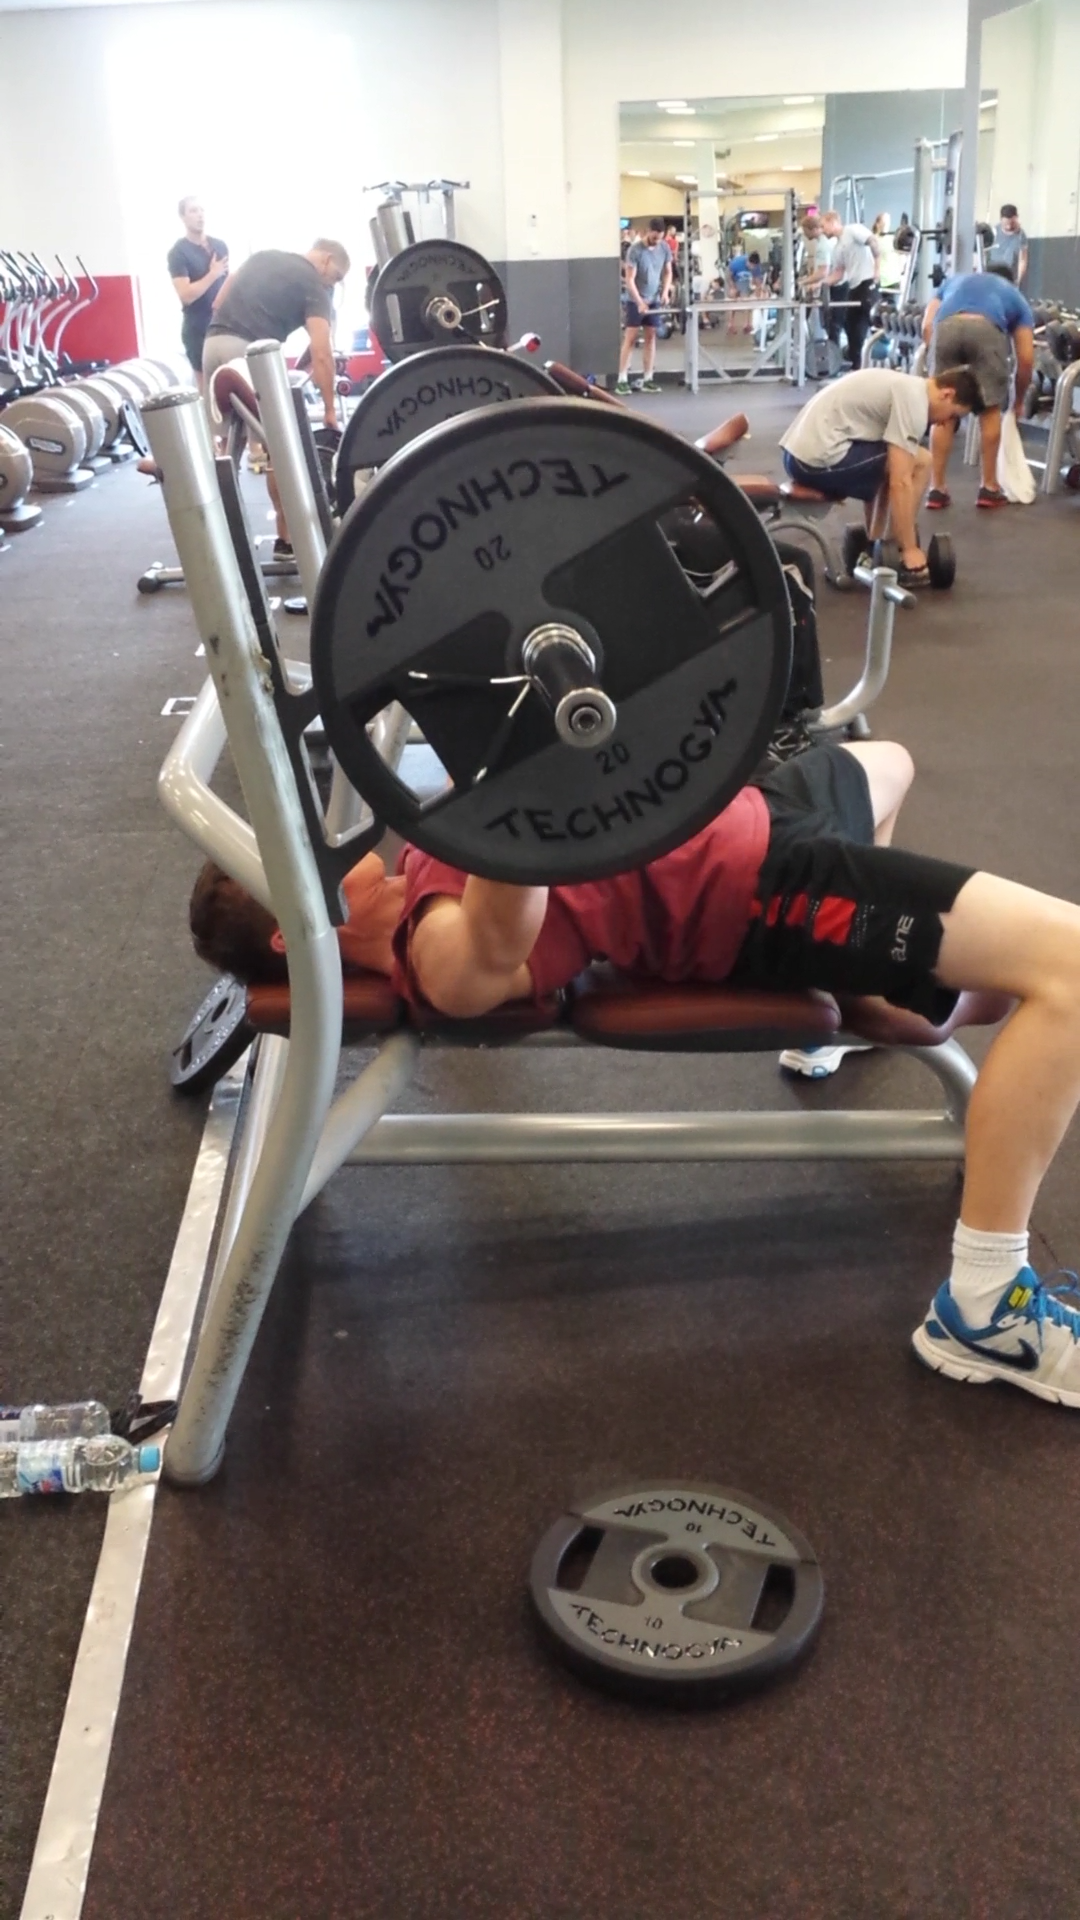
\includegraphics[height=7cm]{intro/images/bench_start}
    }
    \subfigure[Middle]{
            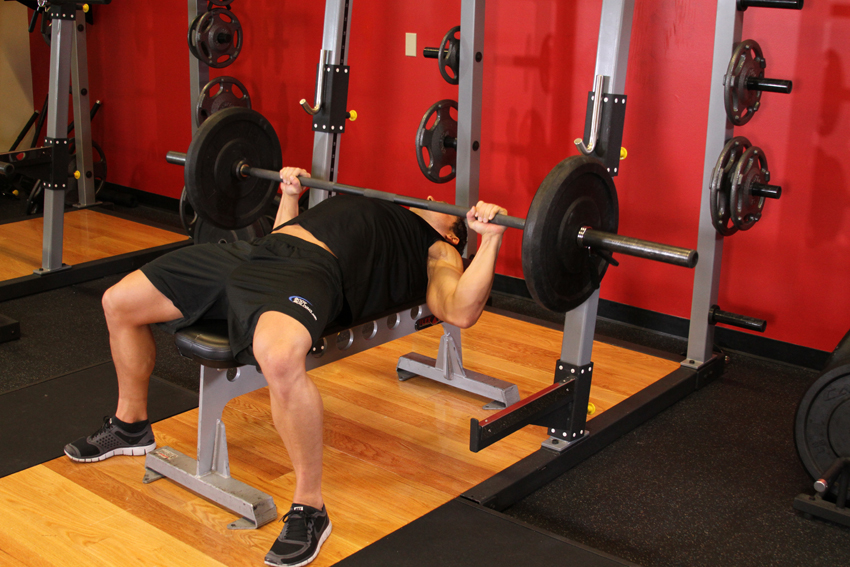
\includegraphics[height=7cm]{intro/images/bench_middle}
    }
    \subfigure[End]{
            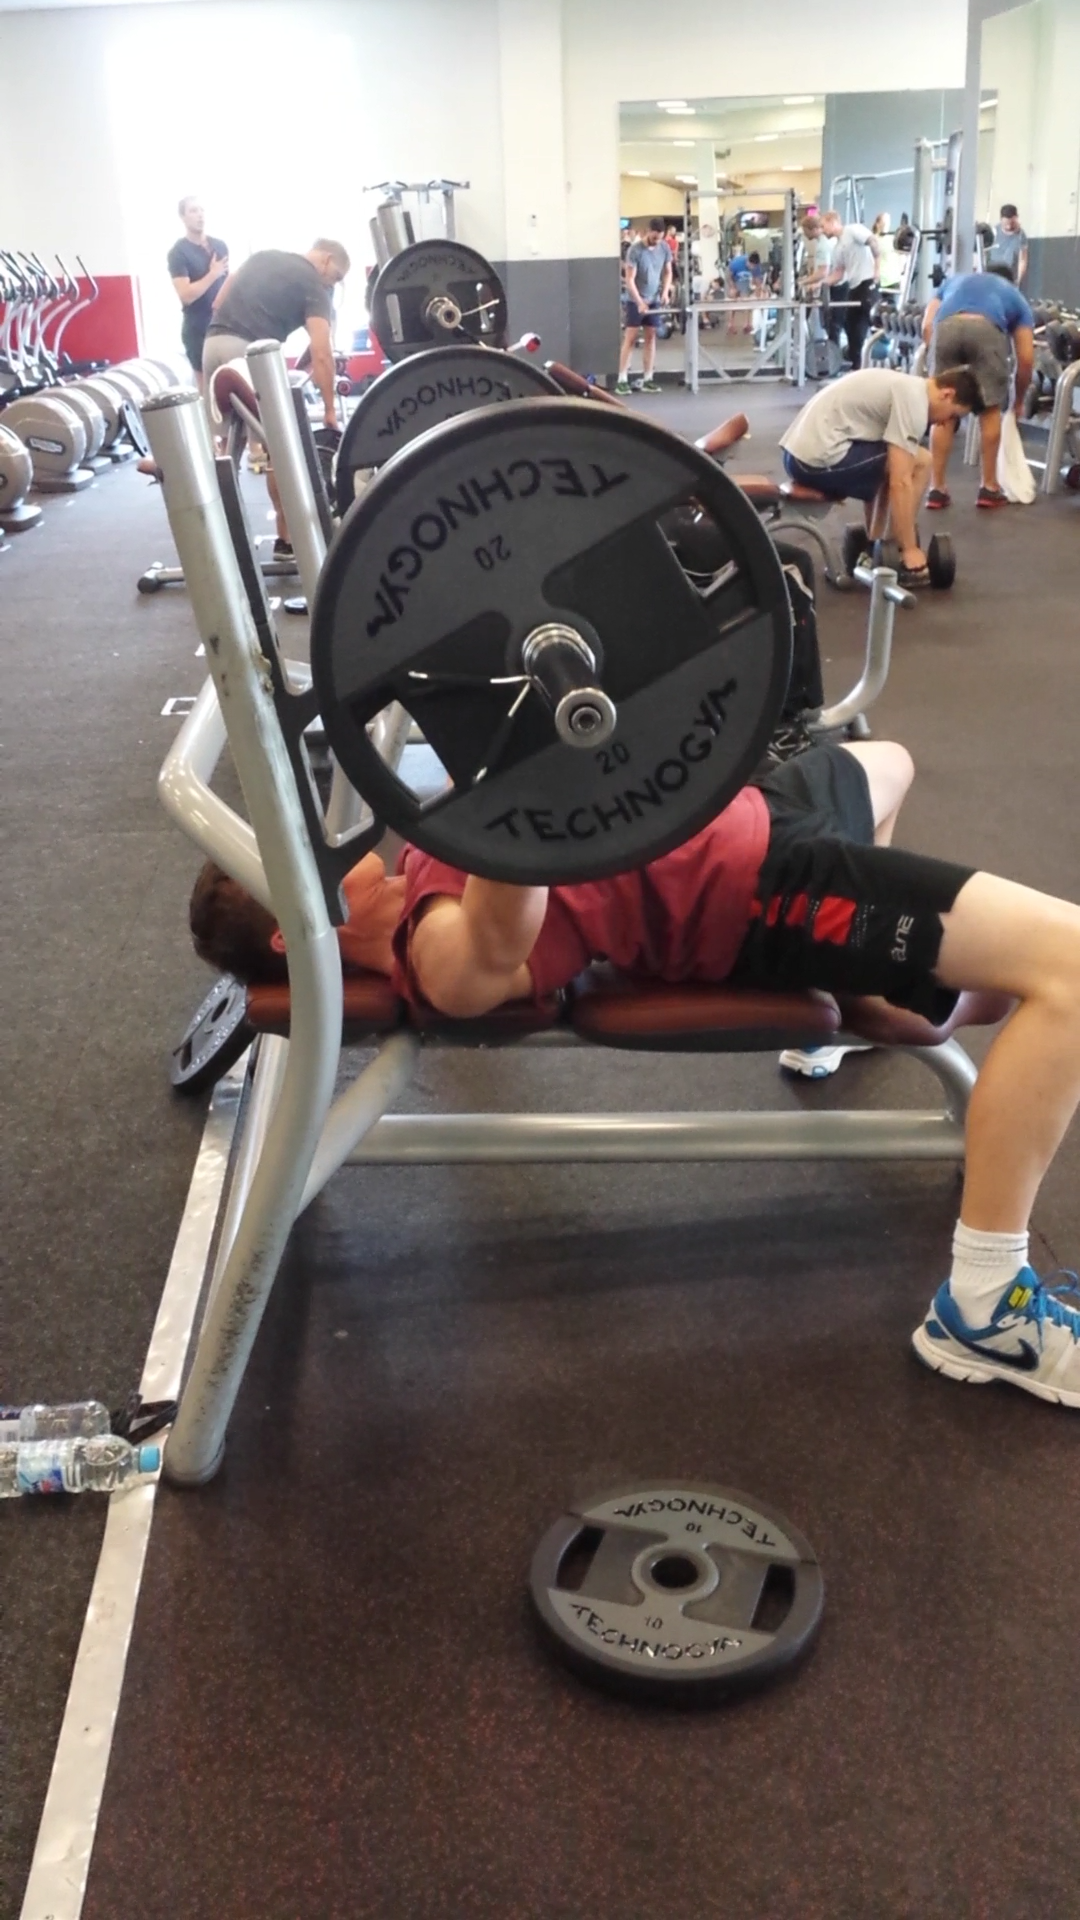
\includegraphics[height=7cm]{intro/images/bench_start}
    }
\caption{The stages of a bench press}
\label{fig:bench_stages}
\end{figure}

The International Powerlifting Federation regulations\cite{ipf} state that during the bench press, the body position of the lifter must not change, ie. the hips, shoulders and head should remain in contact with the bench at all times.